\chapter{Pilas}

\section{Definición de Pila}
Una pila (stack en inglés) es una lista ordinal o estructura de datos en la que el modo de acceso a sus elementos es de tipo LIFO (del inglés Last In First Out, último en entrar, primero en salir) que permite almacenar y recuperar datos. Se aplica en multitud de ocasiones en informática debido a su simplicidad y ordenación implícita en la propia estructura. 

La Figura  \ref{fig:pila-diagrama-clases} muestra la representación gráfica de una pila con sus operaciones fundamentales de apilar (push en inglés) y desapilar o retirar (pos en inglés.).

La pila es muy útil en situaciones cuando los datos deben almacenarse y luego recuperarse en orden inverso.

\begin{figure}
	\centering
		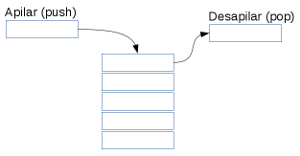
\includegraphics{images/RepresentacionPila}
	\caption{Representación de una Pila}	
	\label{fig:pila-representacion}
\end{figure}

\begin{definicion}[Pila][capPilas:pila]
Una pila (stack en inglés) es una lista ordinal o estructura de datos en la que el modo de acceso a sus elementos es de tipo LIFO (del inglés Last In First Out, último en entrar, primero en salir) que permite almacenar y recuperar datos. FALTA REFERENCIA
\end{definicion}

\section{El TAD Pila}
A continuación se especifica el TAD de la Pila con sus operaciones fundamentales. Las operaciones apilar y desapilar son las más importantes. En seguida la especificación de cada operación del TAD al estilo C.

\begin{lstlisting}[numbers=none, language=C]
TAD Pila [ T ]
{ invariante: TRUE }
Constructoras:
   crearPila: 
Modificadoras:
	apilar: Pila T 
	desapilar: Pila
Analizadoras:
	cima: Pila 
	esVacia: Pila
Destructora:
	destruirPila: Pila

Pila crearPila( void )
/* Crea una pila vacia */
{ post: crearPila =  }

void apilar(Pila pil, T elem)
/* Coloca sobre el tope de la pila el elemento elem */\
{ post: pil = e1, e2, .. elem}

void desapilar(Pila pil)\\
/* Elimina el elemento que se encuentra en el tope de la pila */\\
{ pre: pil =e1, e2, ..en, n > 0 }
{ post: pil =e1, e2, .., en-1 }

T cima(Pila pil )
/* Retorna el elemento que se encuentra en el tope de la pila */
{ pre: n > 0 }
{ post: cima = en }

int esVacia( Pila pil )
/* Informa si la pila esta vacia */
{ post: esVacia = ( pil = ) }

void destruirPila( Pila pil )
/* Destruye la pila retornando toda la memoria ocupada */
{post: pil ha sido destruida }
\end{lstlisting}

\section{Implementación del TAD en Java}
A continuación se muestra una implementación en Java del TAD Pila. Debido a que es una Pila dinámica se utilizan nodos enlazados.  La Figura \ref{fig:pila-digrama-clases} muestra el diagrama de clases.


\begin{figure}
	\centering
		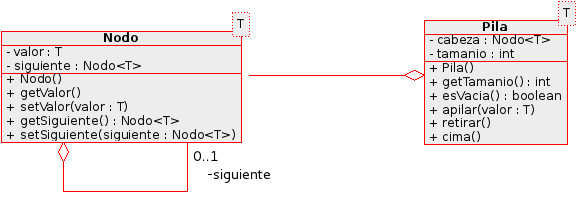
\includegraphics{images/DiagramaClases-Pila}
	\caption{Diagrama de clase de la implementación del TAD Pila}	
	\label{fig:pila-diagrama-clases}
\end{figure}

La implementación involucra básicamente dos clases: Nodo y Pila. 

\begin{lstlisting}[language=Java]
package co.unicauca.pilas;
public class Nodo<T> {
	//Atributo valor de tipo T. Almacena la referencia al objeto que se guarda en el nodo
 	private T valor;
 	//Referencia al siguiente nodo enlazado
 	Nodo<T> siguiente;
	//Constructor por defecto
 	public Nodo() {
 		valor = null;
 		siguiente = null;
 	}
	//Devuelve el valor 
 	public T getValor() {
 		return valor;
 	}
	//Modifica el valor
 	public void setValor(T valor) {
 		this.valor = valor;
 	}
	//Devuelve el atributo siguiente
 	public Nodo<T> getSiguiente() {
 		return siguiente;
 	}
	 //Modifica el atributo siguiente
 	public void setSiguiente(Nodo<T> siguiente) {
 		this.siguiente = siguiente;
 	}
 }
\end{lstlisting}
La clase Nodo representa cada uno de los nodos enlazados que almacenan los objetos que se apilan. Tiene dos atributos, el \textsl{valor} representa el valor que guarda el nodo (línea 4), en este caso es una referencia a un objetivo de tipo T (siendo T un tipo genérico). El atributo \textsl{siguiente} (línea 6), representa la referencia al siguiente nodo. Los demás son únicamente, constructor y getters y setters de cada atributo.

\begin{lstlisting}[language=Java]
package co.unicauca.pilas;
public class Pila<T> {
    //Atributo cabeza, que apunta al tope la pila
 	private Nodo<T> cabeza;
 	//Almacena el total de elemento de la pila
 	private int tamanio;
    //Constructor por defecto
 	public Pila() {
 		cabeza = null;
 		tamanio = 0;
 	}
	//Devuelve el total de elementos de la pila
 	public int getTamanio() {
 		return tamanio;
 	}
	//Verifica si la pila esta vacia
 	public boolean esVacia() {
 		return (cabeza == null)
 	}
	//Apila un elemento nuevo
 	public void apilar(T valor) {
	 	//Crear un nuevo Nodo
 		Nodo<T> nuevo = new Nodo<T>();
	 	//Fijaer el valor dentro del nodo
 		nuevo.setValor(valor);
 		if (esVacia()) {
	 		//Cabeza apunta al nodo nuevo
 			cabeza = nuevo;
 		} else {
	 		//Se enlaza el campo siguiente de nuevo con la cabeza
 			nuevo.setSiguiente(cabeza);
 			//La nueva cabeza de la pila pasa a ser nuevo
 			cabeza = nuevo;
 		}
 		//Incrementa el tamanio porque hay un nuevo elemento en la pila
 		tamanio++;
 	}
	//Elimina un elemento de la pila
 	public void retirar() {
 		if (!esVacia()) {
 			cabeza = cabeza.getSiguiente();
 			tamanio--;
. 		}
 	}
	//Devuelve el elemento almacenado en el tope de la pila
 	public T cima() {
 		if (!esVacia())
 			return cabeza.getValor();
 		else
 			return null;
 	}
 }
\end{lstlisting}

La clase Pila representa la pila como tal con sus operaciones principales de \textsl{apilar} y \textsl{retirar}. 

A continución el código de un Cliente que instancia la Pila que hemos creado. En este caso se almacenan objetos de tipo entero, se apilan algunos números, se imprimen los valores del tope de pila y se desapilan elementos.

\begin{lstlisting}[language=Java]
package co.unicauca.pilas;
public class ClienteMain {
	public static void main(String[] args) {
		//Crear una nueva pila de enteros
		Pila<Integer> pila2 = new Pila<Integer>();
		//Se apilan algunos datos enteros
		pila2.apilar(2);
		pila2.apilar(5);
		pila2.apilar(7);
		System.out.println("El tope de la pila es: " + pila2.cima());
		//Se desapila
		pila2.retirar();
		System.out.println("El tope de la pila es: " + pila2.cima());
		//Se desapila
		pila2.retirar();
		System.out.println("El tope de la pila es: " + pila2.cima());
		//Se desapila, como la pila esta vacia devuelve null
		pila2.retirar();
		System.out.println("El tope de la pila es: " + pila2.cima());
 		//Probar con otra pila, donde se almacenen objetos
 	}
}
\end{lstlisting}

La salida de este programa sería la siguiente.

\begin{lstlisting}[numbers=none]
El tope de la pila es: 7
El tope de la pila es: 5
El tope de la pila es: 2
El tope de la pila es: null
\end{lstlisting}

